\documentclass{article}

\usepackage[nonatbib,final]{neurips}
\usepackage[backend=biber,style=numeric-comp,doi=false,url=false]{biblatex}
\setlength\bibitemsep{0.5\baselineskip}
\usepackage{bm}
\usepackage{csquotes}
\usepackage[inkscapelatex=false]{svg}

\addbibresource{references.bib}
\graphicspath{{../figs/}}
\svgpath{{../plots/}}

\newcommand{\todo}{\bf \color{blue} [TODO]~}

\makeatletter
\renewcommand{\@noticestring}{
  \centering

}
\makeatother

\input{extra_pkgs}

\usepackage{physics}
\usepackage{mathtools}
\DeclarePairedDelimiter\p{(}{)}
\DeclarePairedDelimiter\n{|}{|}
\DeclarePairedDelimiter\B{[}{]}

\title{Self-Training with Models for Tabular Data}

\author{
    Wei En, Ng \\
    National University of Singapore \\
    \texttt{\href{mailto:ngwe@u.nus.edu}{ngwe@u.nus.edu}}
}

\begin{document}

\maketitle

\section{Introduction}

This report details some preliminary experiments studying self-training
\cite{amini2023selftraining} on tabular data, where tree-based models often outperform
deep learning methods significantly in the typical supervised learning (SL) setting
\cite{shwartz-ziv2021tabular,grinsztajn2022why}.\footnote{%
  Some recent works \cite{gorishniy2023tabr} have claimed to develop deep learning
  models that can outperform tree-based methods such as XGBoost \cite{chen2016xgboost}
  on tabular data.
}

Several general observations have been made on the performance of these methods:
\begin{enumerate}
    \item ($\bm{-}$) Increasing the random search budget for hyperparameters does
    not benefit NNs. \cite{grinsztajn2022why}
    \item ($\bm{-}$) NNs continue to do poorly on datasets with only numerical
    features, although the performance gap is slightly reduced compared to datasets with
    categorical features. \cite{grinsztajn2022why}
    \item ($\bm{+}$) Increasing the number of training samples might reduce the
    performance gap. \cite{grinsztajn2022why}
\end{enumerate}

Furthermore, low-data regimes for tabular data do not appear to be well-studied,
possibly because tree-based models seem to reach near-optimal performance with low
training dataset sizes.\footnote{%
  See Figure \ref{fig:ul_split_vs_l_split} where \texttt{l\_split=0.1} (corr. to 200
  samples) usually produces test accuracies $\pm 5\%$ within that of \texttt{l\_split=1}
  (corr. to 2k samples) across different tree-based models and dataset combinations.
  Note that the original datasets are often much bigger with at least 10k samples, as
  listed in Table \ref{tab:datasets}.
}

A recent theoretical analysis of self-training \cite{wei2022theoretical} argues that it
is possible for deep models to generalise and outperform SL models by denoising
incorrect pseudolabels.\footnote{%
  \todo explain the assumptions made and application only to visual modality
} Inspired by this result, we propose the following guiding question:
\begin{displayquote}
  Can deep learning methods outperform tree-based methods in the low-labelled-data
  regime, given access to a large unlabelled dataset and employing self-training to
  enlarge the training dataset?
\end{displayquote}

Naturally, to answer this question would require an extensive understanding of
self-training, which is difficult even in the vision domain \cite{wei2022theoretical},
and also of the advantanges that deep learning models have in the tabular domain.
This report investigates the following smaller subquestions: \begin{enumerate}
  \item How does self-training vary across classes of models, e.g. ensemble-based
  methods (\texttt{random-forest}), gradient boosting (\texttt{hgbt}) and deep models
  (\texttt{mlp})?
  \item When is self-training stable?
\end{enumerate}

\subsection{Literature Review}

Past works on semi-supervised tree-based models for tabular data include
tree-based models \cite{kemp2003semisupervised,levatic2017semisupervised,
tanha2017semisupervised}, of which \cite{tanha2017semisupervised} proposes a
self-training method on decision tree classifiers, and modern approaches inspired by
successes in deep learning such as VIME \cite{yoon2020vime} and Contrastive Mixup
\cite{darabi2021contrastive}, which both rely on data augmentation.

{\todo will write more on comparing existing approaches}

\section{Methodology}\label{sec:met}

\subsection{Datasets \& Models}

The tabular datasets used for our experiments were picked from benchmarks in
\cite{grinsztajn2022why,shwartz-ziv2021tabular}, selected for their high number of
samples, features and classes, which likely implies a high sample complexity.

\begin{table}[htbp]
  \centering
  \caption{Datasets employed in our experiments.}
  \label{tab:datasets}
  \begin{tabular}{rccccc}
    \toprule
    & \textbf{Samples} & \multicolumn{3}{c}{\textbf{Features}} & \textbf{Classes} \\
    \cmidrule(lr){3-5}
    & & Numerical & Categorical & Total \\
    \midrule
    \small\texttt{jannis} \cite{grinsztajn2022why} & 57.5k & 54 & - & 54 & 2 \\
    \small\texttt{gas-drift}$^a$ \cite{grinsztajn2022why,shwartz-ziv2021tabular}
    & 13.9k & 129 & - & 129 & 6 \\
    \small\texttt{higgs} \cite{grinsztajn2022why,shwartz-ziv2021tabular}
    & 98k & 28 & - & 28 & 2 \\
    \small\texttt{covertype} \cite{shwartz-ziv2021tabular}
    & 581k & 10 & 44 & 54 & 7 \\
    \bottomrule
  \end{tabular}

  \footnotesize{
    $^a$ Abbreviation of \texttt{gas-drift-different-concentrations}.
  }
\end{table}

The models used for our experiments were: \begin{enumerate}
  \item \texttt{hgbt} (Histogram-based Gradient Boosting Classification Tree)
  \item \texttt{mlp} (Multi-layer Perceptron), adapted from
  \cite{gorishniy2021revisiting}
  \item \texttt{random-forest} (Random Forest)
\end{enumerate}
\texttt{hgbt} and \texttt{random-forest} was implemented using
\texttt{HistGradientBoostingClassifier} and \texttt{RandomForestClassifier} in
Scikit-learn v1.3.0 \cite{pedregosa2011scikitlearn} resp., while \texttt{mlp} was
implemented with Pytorch v2.0.1 \cite{paszke2019pytorch}.

\subsection{Train/Test/Val \& Labelled/Unlabelled Split}

We conduct our experiments across different splits, where each split consists of
2k/1k/1k randomly sampled samples as our training/test/validation datasets.

Within the training dataset, we randomly sample labelled (L) and unlabelled (UL) samples
to be used in the experiment by picking proportions \texttt{l\_split},
\texttt{ul\_split} $\in [0, 1]$ resp. such that \texttt{l\_split} $> 0$ and
\texttt{l\_split} $+$ \texttt{ul\_split} $\leq 1$.
For e.g., \texttt{l\_split=0.25} and \texttt{ul\_split=0.05} correspond to 500 L samples
and 100 UL samples resp..\footnote{%
  While the number of validation samples may seem very high compared to the number of L
  samples typically available, we note that the validation dataset is currently only
  used by \texttt{mlp} to adjust its learning rate and reduce the possibility of
  escaping the minima, following the experiments of \cite{grinsztajn2022why} which use
  PyTorch's \texttt{ReduceLROnPlateau}.
  Future experiments can explore the possibility of employing other forms of
  regularisation that do not rely on access to a large validation dataset for a more
  realistic setting.
}

\subsection{Hyperparameter Sweeps}

As we plan to examine models across low-data and high-data regimes on varied datasets,
it is crucial to pick appropriate hyperparameter choices that do not bias the model
towards either regime.\footnote{%
  For e.g., choosing a high value of \texttt{min\_samples\_leaf} for \texttt{hgbt}
  restricts the model to shallow trees on small training datasets, adversely affecting
  performance.
} Additionally, certain hyperparameter choices can lead to very inconsistent performance
on different splits of the dataset, even if the number of L and UL training samples is
the same.

For efficiency, we fix a select choice of hyperparameters for each SL model across all
splits, following this procedure: \begin{enumerate}
  \item Run over 40 sweeps using Optuna \cite{akiba2019optuna}'s Tree-structured
  Parzen Estimator (\texttt{TPESampler}) algorithm, where for each sweep on the SL
  model:
  \begin{enumerate}
    \item Let \texttt{n\_splits=5}.
    \item Compute the harmonic mean of the test accuracy over \texttt{n\_splits} splits
    of the dataset on \texttt{l\_split=0.025} (``small'').
    \item Similarly, compute the harmonic mean for \texttt{l\_split=0.25} (``large'').
  \end{enumerate}
  \item Round off the test accuracies to the nearest percent.
  \item Out of the sweeps lying on the Pareto front, select a sweep with the highest
  test accuracy on \texttt{l\_split=0.25} (``large'').\footnote{%
    This is based on the assumption that the sweep will eventually find a set of
    ``optimal'' hyperparameters which achieve within 0.5\% of the best accuracy on the
    large split, while also performing ``well'' on the small split.
  }
\end{enumerate}
For self-training, we adopted the same hyperparameters used for the base supervised
learning models.

The choice of the harmonic mean penalises inconsistent performance across splits of the
dataset, while the last two steps enable us to select hyperparameters that have room to
improve as the amount of data increases, while still having a close-to-optimal baseline
performance on a small split.

The hyperparameter search space used for each model, as well as plots of the sweep
results, are attached in Appendix \ref{sec:hyperparams_sweep_plots}.

\subsection{Self-training Algorithms}

The versatility of self-training enables the plug-and-play use of most such methods on
any supervised learning method, both within and outside of deep learning, and without
requiring additional loss terms (i.e. self-training does not apply to only methods
using gradient-based optimisation techniques).

A common type of self-training proposed is threshold-based \cite{amini2023selftraining},
where pseudolabels are only adopted into the training dataset if their probability
scores are above a certain threshold.
Although schemes exist to adjust this threshold, in order to avoid issues with model
calibration\footnote{%
  As models are trained over datasets of increasing size, even with a fixed number of
  iterations, the model may still overfit on smaller datasets and produce overly sharp
  predictions.
}, we chose to use an adaptation of curriculum learning to pseudolabelling
\cite{cascante-bonilla2020curriculum}, which picks pseudolabels from the top $20t\%$ of
samples on the $t$th pseudolabelling iteration (for $t \in \{1, \ldots, 5\}$).

\begin{figure}[htbp]
  \centering
  \includegraphics[width=\columnwidth]{curriculum_pseudolabelling.png}
  \caption{
    Illustration of curriculum pseudolabelling from
    \cite{cascante-bonilla2020curriculum}.
    The precise algorithm can be found in Algorithm 1 of
    \cite{cascante-bonilla2020curriculum}.
  }
  \label{fig:curr-pl}
\end{figure}

\section{Results}\label{sec:res}

\subsection{Overall Test Accuracies}

We first conducted self-training experiments on a mix of model/dataset combinations,
assessing the mean test accuracy across the following data regimes: high-L, low-L
high-UL, and low-L low-UL.
(High and low refers to a proportion within $[0.25, 1]$ and $[0, 0.1]$ resp..)

Hyperparameters selected for the experiment are available at Table
\ref{tab:test_acc_hyperparams}.
The plots are available at Figure \ref{fig:ul_split_vs_l_split},
\ref{fig:test_acc_vs_ul_split_low} \& \ref{fig:test_acc_vs_ul_split_high}.
A summary of the mean and standard deviation of the test accuracies is provided in Table
\ref{tab:test_acc_summary} for easier comparison between model performance.

\begin{table}[htbp]
  \centering
  \caption{Hyperparameters selected for each dataset/model combination.}
  \label{tab:test_acc_hyperparams}
  \small
  \begin{tabular}{rccccccc}
    \toprule
    & \multicolumn{3}{c}{\normalsize\texttt{hgbt}} & \multicolumn{2}{c}{\normalsize\texttt{mlp}} & \multicolumn{2}{c}{\normalsize\texttt{random-forest}} \\
    \cmidrule(lr){2-4}
    \cmidrule(lr){5-6}
    \cmidrule(lr){7-8}
    & \texttt{lr} & \texttt{max\_depth} & \tiny\texttt{min\_samples\_leaf} & \texttt{layer\_size} & \texttt{lr} & \texttt{max\_depth} & \tiny\texttt{min\_samples\_leaf} \\
    \midrule
    \texttt{jannis} & 0.05 & - & 5 & 256 & 0.016 & - & 3 \\
    \texttt{gas-drift} & 0.025 & 2 & 5 & 192 & 0.04 & - & 1 \\
    \texttt{higgs} & 0.05 & 2 & 2 & 192 & 0.032 & - & 5 \\
    \texttt{covertype} & 0.15 & - & 3 & 192 & 0.04 & - & 1 \\
    \bottomrule
  \end{tabular}
\end{table}

Generally, we find that curriculum self-training does not offer much benefit over
supervised learning, although we have yet to implement any form of input consistency
regularisation.\footnote{%
  The theoretical results of \cite{wei2022theoretical} apply only when input consistency
  regularisation is applied to the training process.
}
Notably, in the low-L data regime, incorporating high-UL data can occasionally lead to
trials with very poor performance, although self-training produces comparable results
most of the time (see top row of matrices in Table \ref{tab:test_acc_summary}, which
often has high standard deviations at the top right).
We study this phenomenon in more detail under Section \ref{sec:det_anal_jannis_mlp}.

Lastly, we attach interactive parallel coordinate plots showing how validation accuracy
changes over pseudolabelling iterations.
For ease of viewing, it is recommended to select specific regions of the graph, e.g. to
see how all experiments performed on a single split, you can select
\texttt{args.seed=0}, \texttt{split.l\_split=0.025}, \texttt{split.ul\_split=0.25}.
{
  \small
  \begin{enumerate}
    \item \texttt{jannis}: \begin{enumerate}
      \item \texttt{hgbt}: \url{https://api.wandb.ai/links/wei2912/52kfpcnd}
      \item \texttt{mlp}: \url{https://wandb.ai/wei2912/ethz-ssl-tabular_jannis/reports/-20230804-Parallel-Coordinate-Plots-mlp---Vmlldzo1MDU0ODM2?accessToken=nqsx9rdqqeejs3fzdnf1x1oo1n8wlfqhe5yx4s6i4oaiz6djm742t2gqactp66ps}
      \item \texttt{random-forest}: \url{https://wandb.ai/wei2912/ethz-ssl-tabular_jannis/reports/-20230804-Parallel-Coordinate-Plots-random-forest---Vmlldzo1MDU0ODQy?accessToken=nywqnqx9cwx1sib3361au2ynljiba3tgj9d9d5064rejzrcn8nkoypfitvrbhs1x}
    \end{enumerate}
    \item \texttt{gas-drift}: \begin{enumerate}
      \item \texttt{hgbt}: \url{https://api.wandb.ai/links/wei2912/5ljhsi70}
      \item \texttt{mlp}: \url{https://api.wandb.ai/links/wei2912/mcdsxevg}
      \item \texttt{random-forest}: \url{https://api.wandb.ai/links/wei2912/fld4y2bj}
    \end{enumerate}
    \item \texttt{higgs}: \begin{enumerate}
      \item \texttt{hgbt}: \url{https://wandb.ai/wei2912/ethz-ssl-tabular_higgs/reports/-20230804-Parallel-Coordinate-Plots-hgbt---Vmlldzo1MDU0ODQ5?accessToken=mmunbdr38oqrjxy8cx33va19xfflkdo7d95rxmvcnhf4uw32gdrec6prmj5pj3ny}
      \item \texttt{mlp}: \url{https://wandb.ai/wei2912/ethz-ssl-tabular_higgs/reports/-20230804-Parallel-Coordinate-Plots-mlp---Vmlldzo1MDU0OTgx?accessToken=0klorbel8nf1shcw6cu2djl6hb6cmbq3sikh79n3qzw788tjwhkifo6cw24lcwn7}
      \item \texttt{random-forest}: \url{https://api.wandb.ai/links/wei2912/kcp3hgny}
    \end{enumerate}
    \item \texttt{covertype}: \begin{enumerate}
      \item \texttt{hgbt}: \url{https://wandb.ai/wei2912/ethz-ssl-tabular_covertype/reports/-20230804-Parallel-Coordinate-Plots-hgbt---Vmlldzo1MDU0Njkz?accessToken=8uejk4mwds8zbghhx799fejblqz1o3z3dhkz6o48jfk6hcncsx1et7n264s5jatm}
      \item \texttt{mlp}: \url{https://wandb.ai/wei2912/ethz-ssl-tabular_covertype/reports/-20230804-Parallel-Coordinate-Plots-mlp---Vmlldzo1MDU0Njg1?accessToken=lyt6ngnatcslorp5d02biv61eo4mso0t34j0bea6ledq5787of3ygnjok0vy03j4}
      \item \texttt{random-forest}: \url{https://wandb.ai/wei2912/ethz-ssl-tabular_covertype/reports/-20230804-Parallel-Coordinate-Plots-random-forest---Vmlldzo1MDU0NTA5?accessToken=z1ac8yvyfv3m8i24711z8wmpae2h09jo0xsy2wrpurp3i3h6ute802kh80gg9s4y}
    \end{enumerate}
  \end{enumerate}
}

\begin{figure}[htbp]
  \centering
  \includesvg[width=\columnwidth]{test_accs/jannis_ul_split_vs_l_split.svg}
  \includesvg[width=\columnwidth]{test_accs/gas-drift-different-concentrations_ul_split_vs_l_split.svg}
  \includesvg[width=\columnwidth]{test_accs/higgs_ul_split_vs_l_split.svg}
  \includesvg[width=\columnwidth]{test_accs/covertype_ul_split_vs_l_split.svg}
  \caption{Test accuracy (acc.) across different splits.}
  \label{fig:ul_split_vs_l_split}
\end{figure}

\begin{figure}[htbp]
  \centering
  \includesvg[width=\columnwidth]{test_accs/jannis_test_acc_vs_ul_split_low.svg}
  \includesvg[width=\columnwidth]{test_accs/gas-drift-different-concentrations_test_acc_vs_ul_split_low.svg}
  \includesvg[width=\columnwidth]{test_accs/higgs_test_acc_vs_ul_split_low.svg}
  \includesvg[width=\columnwidth]{test_accs/covertype_test_acc_vs_ul_split_low.svg}
  \caption{
    Test accuracy (acc.) across multiple splits in the low unlabelled (UL) data regime.
  }
  \label{fig:test_acc_vs_ul_split_low}
\end{figure}

\begin{figure}[htbp]
  \centering
  \includesvg[width=\columnwidth]{test_accs/jannis_test_acc_vs_ul_split_high.svg}
  \includesvg[width=\columnwidth]{test_accs/gas-drift-different-concentrations_test_acc_vs_ul_split_high.svg}
  \includesvg[width=\columnwidth]{test_accs/higgs_test_acc_vs_ul_split_high.svg}
  \includesvg[width=\columnwidth]{test_accs/covertype_test_acc_vs_ul_split_high.svg}
  \caption{
    Test accuracy (acc.) across multiple splits in the high unlabelled (UL) data regime.
  }
  \label{fig:test_acc_vs_ul_split_high}
\end{figure}

\begin{table}[htbp]
  \centering
  \caption{
    Test accuracy (acc.) over five trials with mean and standard deviation.
    Within each matrix: from left to right, \texttt{ul\_split} $=$ 0 (SL), 0.25
    (high-UL); from top to bottom, \texttt{l\_split} $=$ 0.025 (low-L), 0.25 (high-L).
  }
  \label{tab:test_acc_summary}
  \begin{tabular}{rccc}
    \toprule
    & \texttt{hgbt} & \texttt{mlp} & \texttt{random-forest} \\
    \midrule
    \small\texttt{jannis}
    & \begin{minipage}[b]{0.25\columnwidth}
      \centering
      \begin{tabular}{r@{\hskip 0.1in}l}
        $62.7 \pm 6.1$ & $62.6 \pm 4.1$ \\
        $71.9 \pm 1.6$ & $71.0 \pm 2.1$ \\
      \end{tabular}
    \end{minipage}
    & \begin{minipage}[b]{0.25\columnwidth}
      \centering
      \begin{tabular}{r@{\hskip 0.1in}l}
        $64.7 \pm 4.4$ & $63.2 \pm 7.6$ \\
        $70.0 \pm 1.0$ & $70.7 \pm 0.9$ \\
      \end{tabular}
    \end{minipage}
    & \begin{minipage}[b]{0.25\columnwidth}
      \centering
      \begin{tabular}{r@{\hskip 0.1in}l}
        $66.1 \pm 3.9$ & $62.1 \pm 3.8$ \\
        $71.6 \pm 1.6$ & $69.8 \pm 1.9$ \\
      \end{tabular}
    \end{minipage} \\ \addlinespace
    \small\texttt{gas-drift}
    & \begin{minipage}[b]{0.25\columnwidth}
      \centering
      \begin{tabular}{r@{\hskip 0.1in}l}
        $65.3 \pm 3.7$ & $64.5 \pm 2.2$ \\
        $94.7 \pm 0.4$ & $95.0 \pm 0.7$ \\
      \end{tabular}
    \end{minipage}
    & \begin{minipage}[b]{0.25\columnwidth}
      \centering
      \begin{tabular}{r@{\hskip 0.1in}l}
        $76.1 \pm 2.9$ & $66.0 \pm 7.0$ \\
        $97.0 \pm 0.1$ & $97.2 \pm 0.4$ \\
      \end{tabular}
    \end{minipage}
    & \begin{minipage}[b]{0.25\columnwidth}
      \centering
      \begin{tabular}{r@{\hskip 0.1in}l}
        $67.5 \pm 3.4$ & $64.4 \pm 5.3$ \\
        $93.1 \pm 0.8$ & $92.9 \pm 1.3$ \\
      \end{tabular}
    \end{minipage} \\ \addlinespace
    \small\texttt{higgs}
    & \begin{minipage}[b]{0.25\columnwidth}
      \centering
      \begin{tabular}{r@{\hskip 0.1in}l}
        $54.8 \pm 2.1$ & $53.0 \pm 1.8$ \\
        $65.6 \pm 1.7$ & $64.0 \pm 1.2$ \\
      \end{tabular}
    \end{minipage}
    & \begin{minipage}[b]{0.25\columnwidth}
      \centering
      \begin{tabular}{r@{\hskip 0.1in}l}
        $52.1 \pm 2.7$ & $51.5 \pm 2.3$ \\
        $54.9 \pm 2.9$ & $53.3 \pm 3.3$ \\
      \end{tabular}
    \end{minipage}
    & \begin{minipage}[b]{0.25\columnwidth}
      \centering
      \begin{tabular}{r@{\hskip 0.1in}l}
        $53.8 \pm 2.7$ & $51.5 \pm 3.2$ \\
        $65.8 \pm 0.9$ & $62.5 \pm 1.4$ \\
      \end{tabular}
    \end{minipage} \\ \addlinespace
    \small\texttt{covertype}
    & \begin{minipage}[b]{0.25\columnwidth}
      \centering
      \begin{tabular}{r@{\hskip 0.1in}l}
        $52.6 \pm 2.4$ & $52.0 \pm 3.8$ \\
        $68.1 \pm 0.8$ & $67.4 \pm 1.2$ \\
      \end{tabular}
    \end{minipage}
    & \begin{minipage}[b]{0.25\columnwidth}
      \centering
      \begin{tabular}{r@{\hskip 0.1in}l}
        $49.8 \pm 2.4$ & $42.2 \pm 6.9$ \\
        $59.7 \pm 6.2$ & $62.5 \pm 1.3$ \\
      \end{tabular}
    \end{minipage}
    & \begin{minipage}[b]{0.25\columnwidth}
      \centering
      \begin{tabular}{r@{\hskip 0.1in}l}
        $52.8 \pm 2.6$ & $45.0 \pm 2.6$ \\
        $69.3 \pm 1.3$ & $68.4 \pm 1.2$ \\
      \end{tabular}
    \end{minipage} \\
    \bottomrule
  \end{tabular}
\end{table}

\clearpage
\subsection{Detailed Analysis of \texttt{jannis} with \texttt{mlp}}
\label{sec:det_anal_jannis_mlp}

In Figure \ref{fig:par_coords_jannis_mlp}, we observed that for \texttt{l\_split=0.025},
some runs perform at reasonable accuracies while a few runs (see dark blue curves)
experienced a collapse in test accuracies to 50\%.

Curiously, such runs often have an initial validation accuracy (with the model trained
on only the L dataset) comparable to that of other runs ($> 60\%$), but after a few
pseudolabelling iterations (trained on 80-100\% of the pseudolabelled UL dataset),
collapse to $\sim 50\%$ validation accuracy.
As \texttt{jannis} is a binary classification problem, this effectively means the models
are as good as random.

This phenomenon appears to occur more frequently in low-L high-UL data regimes, as
compared to low-L low-UL, although more experiments are required to verify this.

\begin{figure}[htbp]
  \centering
  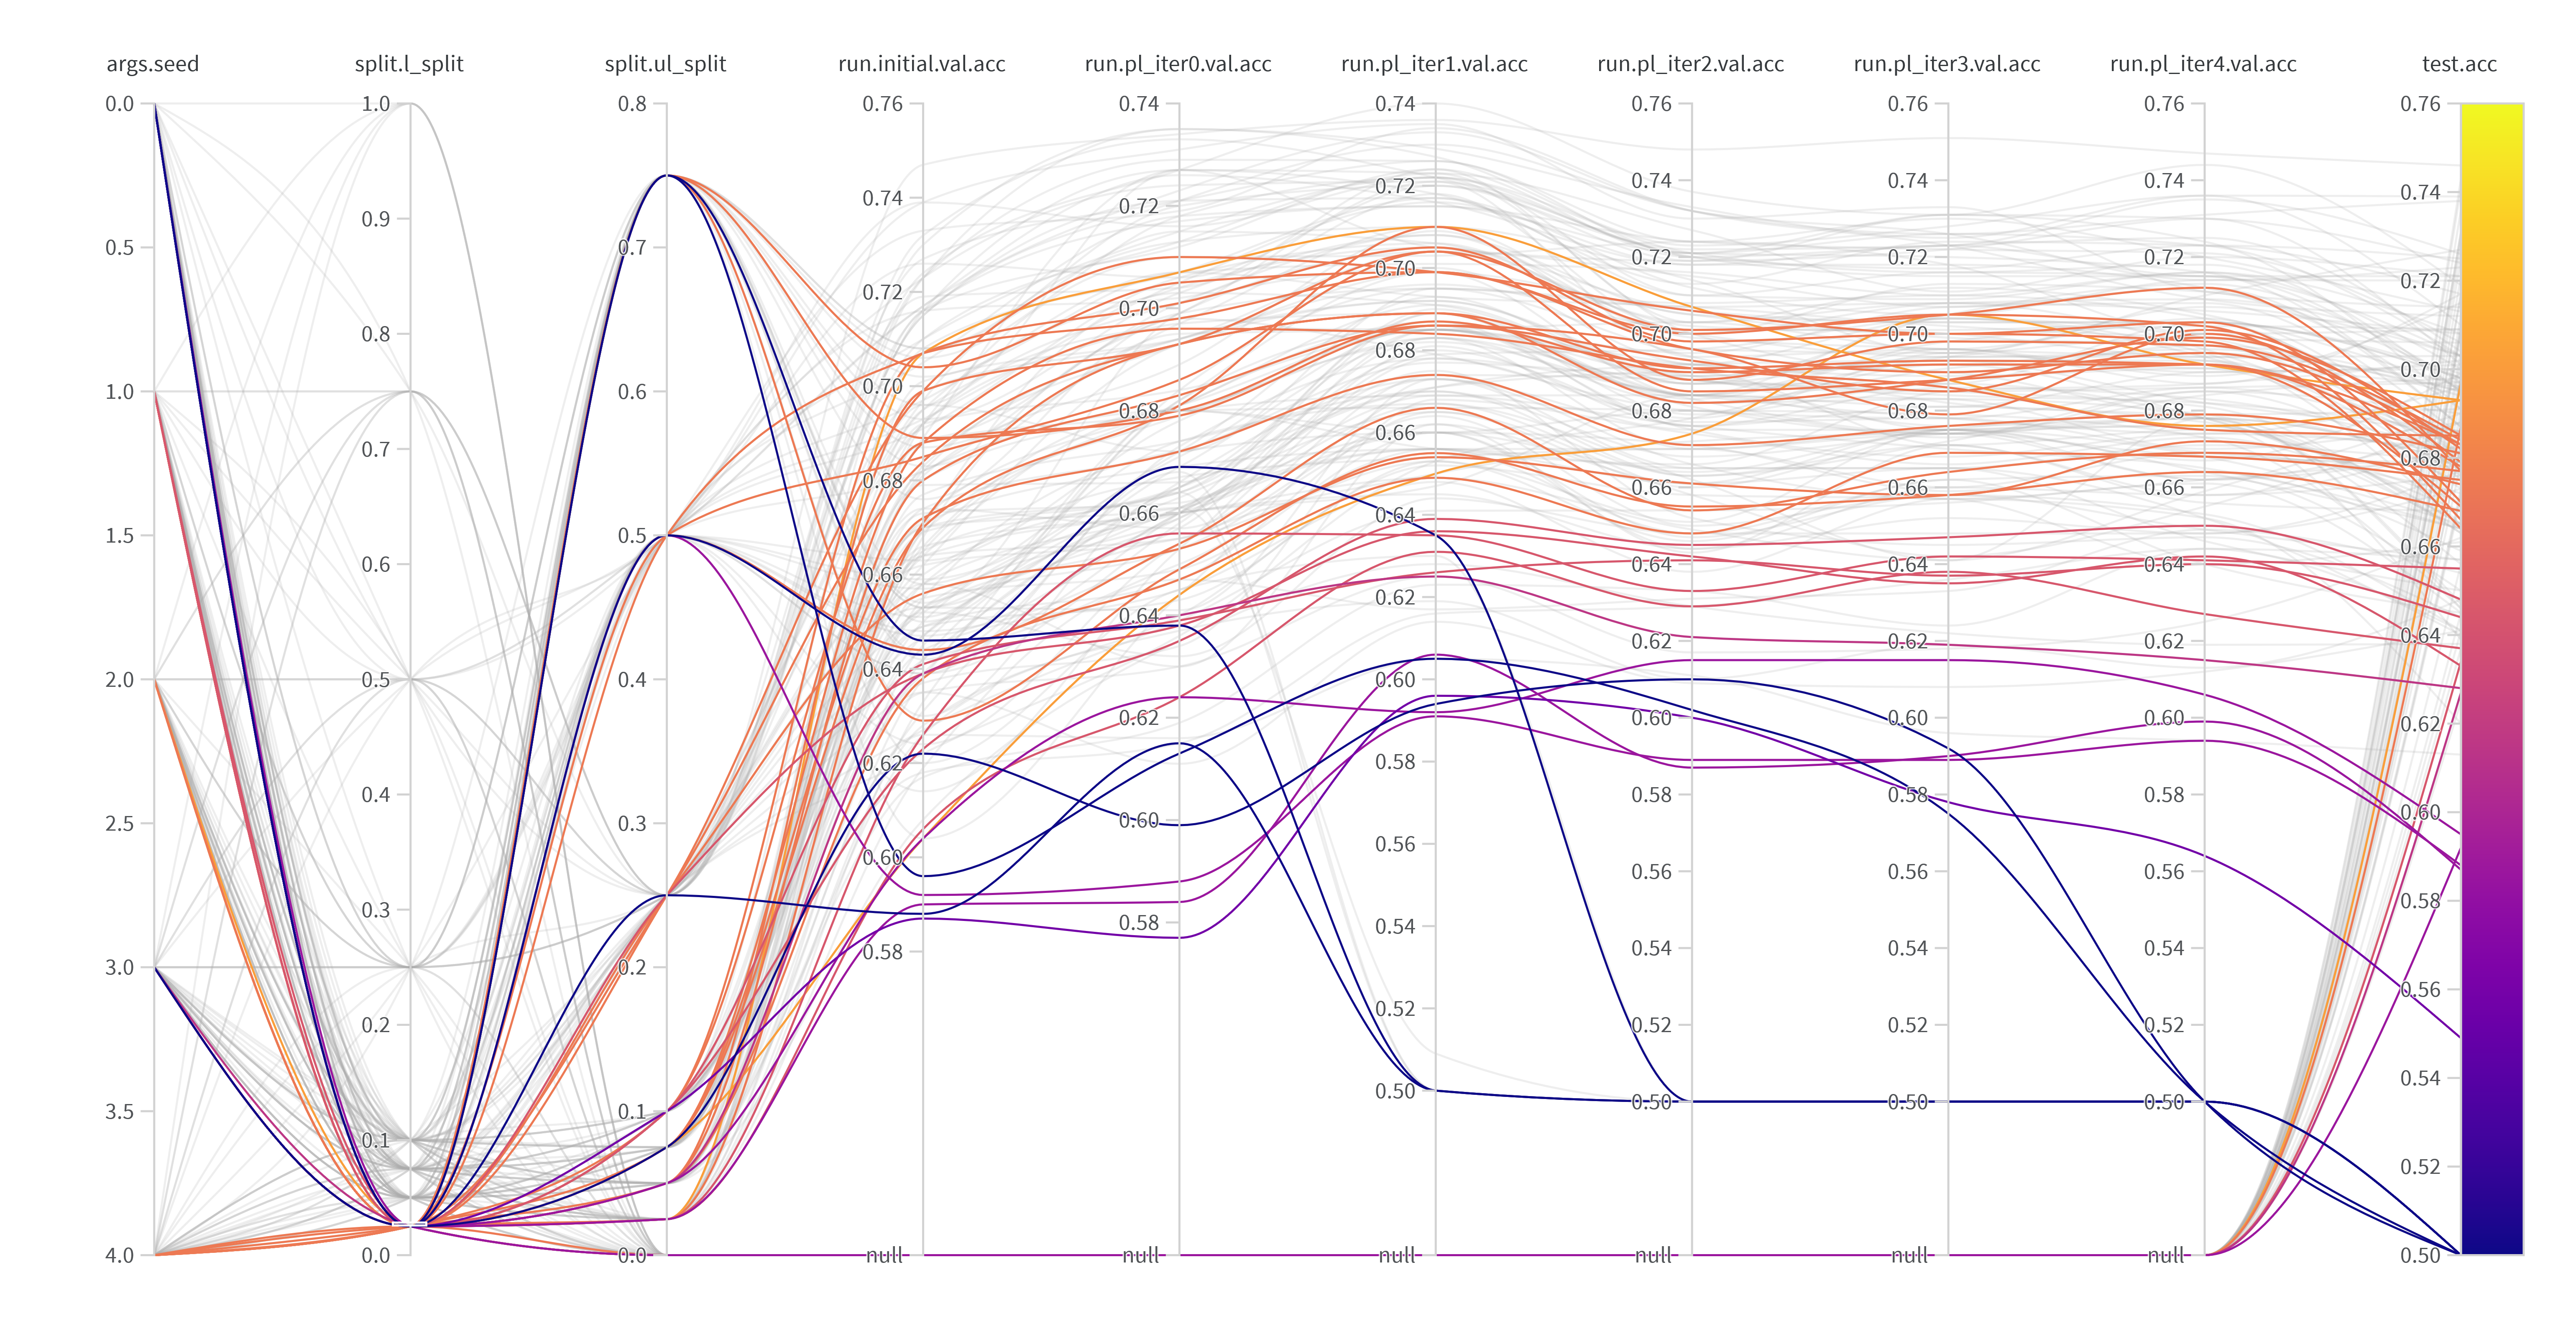
\includegraphics[width=\columnwidth]{par_coords_jannis_mlp.png}
  \caption{Parallel coordinate plot for \texttt{jannis}/\texttt{mlp} with
  \texttt{l\_split=0.025}, available at
  {\small\url{https://wandb.ai/wei2912/ethz-ssl-tabular_jannis/reports/-20230804-Parallel-Coordinate-Plots-mlp---Vmlldzo1MDU0ODM2?accessToken=nqsx9rdqqeejs3fzdnf1x1oo1n8wlfqhe5yx4s6i4oaiz6djm742t2gqactp66ps}}.}
  \label{fig:par_coords_jannis_mlp}
\end{figure}

We conducted additional experiments to examine if the reason for the collapse in
validation accuracy is solely due to dataset label noise:
\begin{enumerate}
  \item Setting \texttt{seed=5}, \texttt{l\_split=0.05}, \texttt{ul\_split=0.75} (such
  that all experiments are provided the same dataset split), we identified a single
  trial which collapsed to 54.4\% validation accuracy and computed the dataset label
  accuracy (\texttt{l\_pl\_acc}) of 64.1\% on the 5th and final pseudolabelling
  iteration (\texttt{pl\_iter4}), which pseudolabels the entire UL dataset.
  This pseudolabelled dataset is used to train the final model from scratch.
  \item Afterwards, we simulated 40 trials of a ``fake'' self-training method, which
  takes the labels of the entire UL dataset and performs random corruptions to achieve a
  similar dataset label accuracy, before training a new model on this dataset.
\end{enumerate}
On 40 trials of the ``fake'' self-training method, we found that all runs achieved
$> 59\%$ validation accuracy, significantly higher than that of the single trial at
54.4\%.
This suggests that the label noise generated by pseudolabelling may have stronger
adversarial effects than uniform label noise.
Consequently, curriculum self-training in the low-L high-UL data regime might require
modifications to stabilise the training process.

\begin{figure}[htbp]
  \centering
  \includegraphics[width=\columnwidth]{par_coords_jannis_mlp_simul_noise.png}
  \caption{Parallel coordinate plot for \texttt{jannis}/\texttt{mlp} with
  \texttt{l\_split=0.05} and \texttt{ul\_split=0.75} over the same dataset split.
  Experiments are still preliminary and not yet available for viewing.}
  \label{fig:par_coords_jannis_mlp_simul_noise}
\end{figure}

\clearpage
\printbibliography

\clearpage
\appendix

\section{Hyperparameter Sweep Plots}
\label{sec:hyperparams_sweep_plots}

\begin{table}[htbp]
  \centering
  \caption{Hyperparameter search space for \texttt{hgbt}.}
  \label{tab:hyperparams_spaces_hgbt}
  \small
  \begin{tabular}{ccc}
    \toprule
    \texttt{lr} & \texttt{max\_depth} & \small\texttt{min\_samples\_leaf} \\
    \midrule
    0.05..0.5 (\texttt{step=0.05})
    & \texttt{None}, 2, 3, 4
    & 1..5 (\texttt{log=True}) \\
    \bottomrule
  \end{tabular}
\end{table}

\begin{table}[htbp]
  \centering
  \caption{Hyperparameter search space for \texttt{mlp}.}
  \label{tab:hyperparams_spaces_mlp}
  \small
  \begin{tabular}{ccccc}
    \toprule
    \texttt{batch\_size} & \texttt{layer\_size} & \texttt{lr} & \texttt{n\_block} & \texttt{n\_iter} \\
    \midrule
    128
    & 64..256 (\texttt{step=64})
    & 0.004..0.04 (\texttt{step=0.004})
    & 4
    & 1000 \\
    \bottomrule
  \end{tabular}
\end{table}

\begin{table}[htbp]
  \centering
  \caption{Hyperparameter search space for \texttt{random-forest}.}
  \label{tab:hyperparams_spaces_random_forest}
  \small
  \begin{tabular}{ccc}
    \toprule
    \texttt{max\_depth} & \small\texttt{min\_samples\_leaf} & \texttt{n\_estimators} \\
    \midrule
    \texttt{None}, 2, 3, 4 & 1..5 (\texttt{log=True}) & 100 \\
    \bottomrule
  \end{tabular}
\end{table}

\begin{figure}[htbp]
  \centering
  \includesvg[width=0.8\columnwidth]{sweep_pareto/jannis_hgbt.svg}
  \includesvg[width=0.8\columnwidth]{sweep_pareto/jannis_mlp.svg}
  \includesvg[width=0.8\columnwidth]{sweep_pareto/jannis_random-forest.svg}
  \caption{
    Harmonic mean of test accuracy (acc.) over five splits, across different
    hyperparameter sweeps on \texttt{jannis}.
  }
  \label{fig:sweep_pareto_jannis}
\end{figure}

\begin{figure}[htbp]
  \centering
  \includesvg[width=0.8\columnwidth]{sweep_pareto/gas-drift-different-concentrations_hgbt.svg}
  \includesvg[width=0.8\columnwidth]{sweep_pareto/gas-drift-different-concentrations_mlp.svg}
  \includesvg[width=0.8\columnwidth]{sweep_pareto/gas-drift-different-concentrations_random-forest.svg}
  \caption{
    Harmonic mean of test accuracy (acc.) over five splits, across different
    hyperparameter sweeps on \texttt{gas-drift}.
  }
  \label{fig:sweep_pareto_gas-drift-different-concentrations}
\end{figure}

\begin{figure}[htbp]
  \centering
  \includesvg[width=0.8\columnwidth]{sweep_pareto/higgs_hgbt.svg}
  \includesvg[width=0.8\columnwidth]{sweep_pareto/higgs_mlp.svg}
  \includesvg[width=0.8\columnwidth]{sweep_pareto/higgs_random-forest.svg}
  \caption{
    Harmonic mean of test accuracy (acc.) over five splits, across different
    hyperparameter sweeps on \texttt{higgs}.
  }
  \label{fig:sweep_pareto_higgs}
\end{figure}

\begin{figure}[htbp]
  \centering
  \includesvg[width=0.8\columnwidth]{sweep_pareto/covertype_hgbt.svg}
  \includesvg[width=0.8\columnwidth]{sweep_pareto/covertype_mlp.svg}
  \includesvg[width=0.8\columnwidth]{sweep_pareto/covertype_random-forest.svg}
  \caption{
    Harmonic mean of test accuracy (acc.) over five splits, across different
    hyperparameter sweeps on \texttt{covertype}.
  }
  \label{fig:sweep_pareto_covertype}
\end{figure}

\end{document}
